% !TEX program = pdflatex

\documentclass{standalone}
\usepackage[utf8]{inputenc}

\usepackage{amsmath}
\usepackage{tikz-feynman}


\newcommand{\pbar}[1]{\overset{\textbf{\fontsize{4pt}{4pt}\selectfont(---)}}{#1}}

\begin{document}

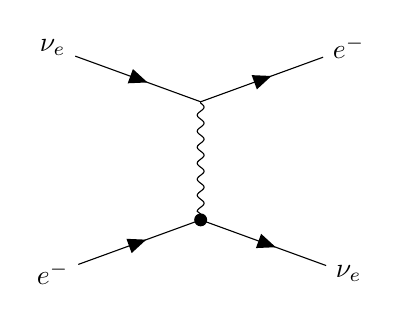
\begin{tikzpicture}

\def\flen{2}
\def\boslen{1.5}
\def\fang{20}

\begin{feynman}
    % \path (170:2) node (i1) {$\nu_e$} -- (0, 0) node (v1)  -- (10:2) node (f1) {$e^-$};
    \vertex (v1) at (0, \boslen);
    \vertex (i1) at ($(v1) + (180-\fang:\flen)$) {$\nu_e$};
    \vertex (f1) at ($(v1) + (\fang:\flen)$) {$e^-$};
    
    \vertex [dot] (v2) at (0, 0) {};
    \vertex (i2) at ($(v2) + (\fang-180:\flen)$) {$e^-$};
    \vertex (f2) at ($(v2) + (-\fang:\flen)$) {$\nu_e$};
    
    \diagram*{
        (i1) -- [fermion] (v1) -- [fermion] (f1),
        (i2) -- [fermion] (v2) -- [fermion] (f2),
        (v1) -- [boson] (v2)
    };
\end{feynman}

\end{tikzpicture}


\end{document}